\subsection{トポロジ}
グループは,ある数のセンサノードから構成される.グループのトポロジは,グループ内での通信とGLノードとGWノードの通信と2種類ある.ノード間通信は,前者にBLE,後者にLoRaWANを用いる.

\begin{figure}[]
    \begin{center}
    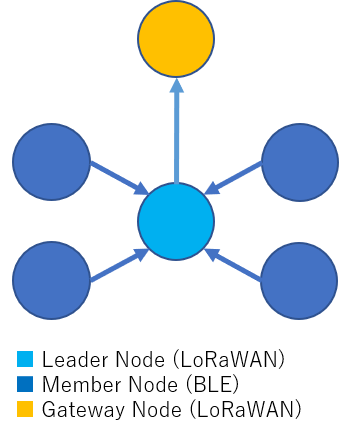
\includegraphics[width=5cm]{figures/グループ化のトポロジ.png}
    \caption{グループ化のトポロジ}
    \label{fig:group_topology}
    \end{center}
\end{figure}